\pagestyle{circuito}
\label{circuito}
%\begin{textblock*}{5.625in}(0pt,0pt)%
%\vspace*{-3.49cm}
%\hspace*{-2.76cm}\includegraphics*[width=175.2mm]{./propagandas/CIRCUITO.pdf}
%\end{textblock*}

\begin{center}
\hspace*{-3.6cm}\raisebox{5cm}{\rotatebox[origin=t]{90}{\huge\textbf{Lançamento}}}
\hspace*{3.1cm}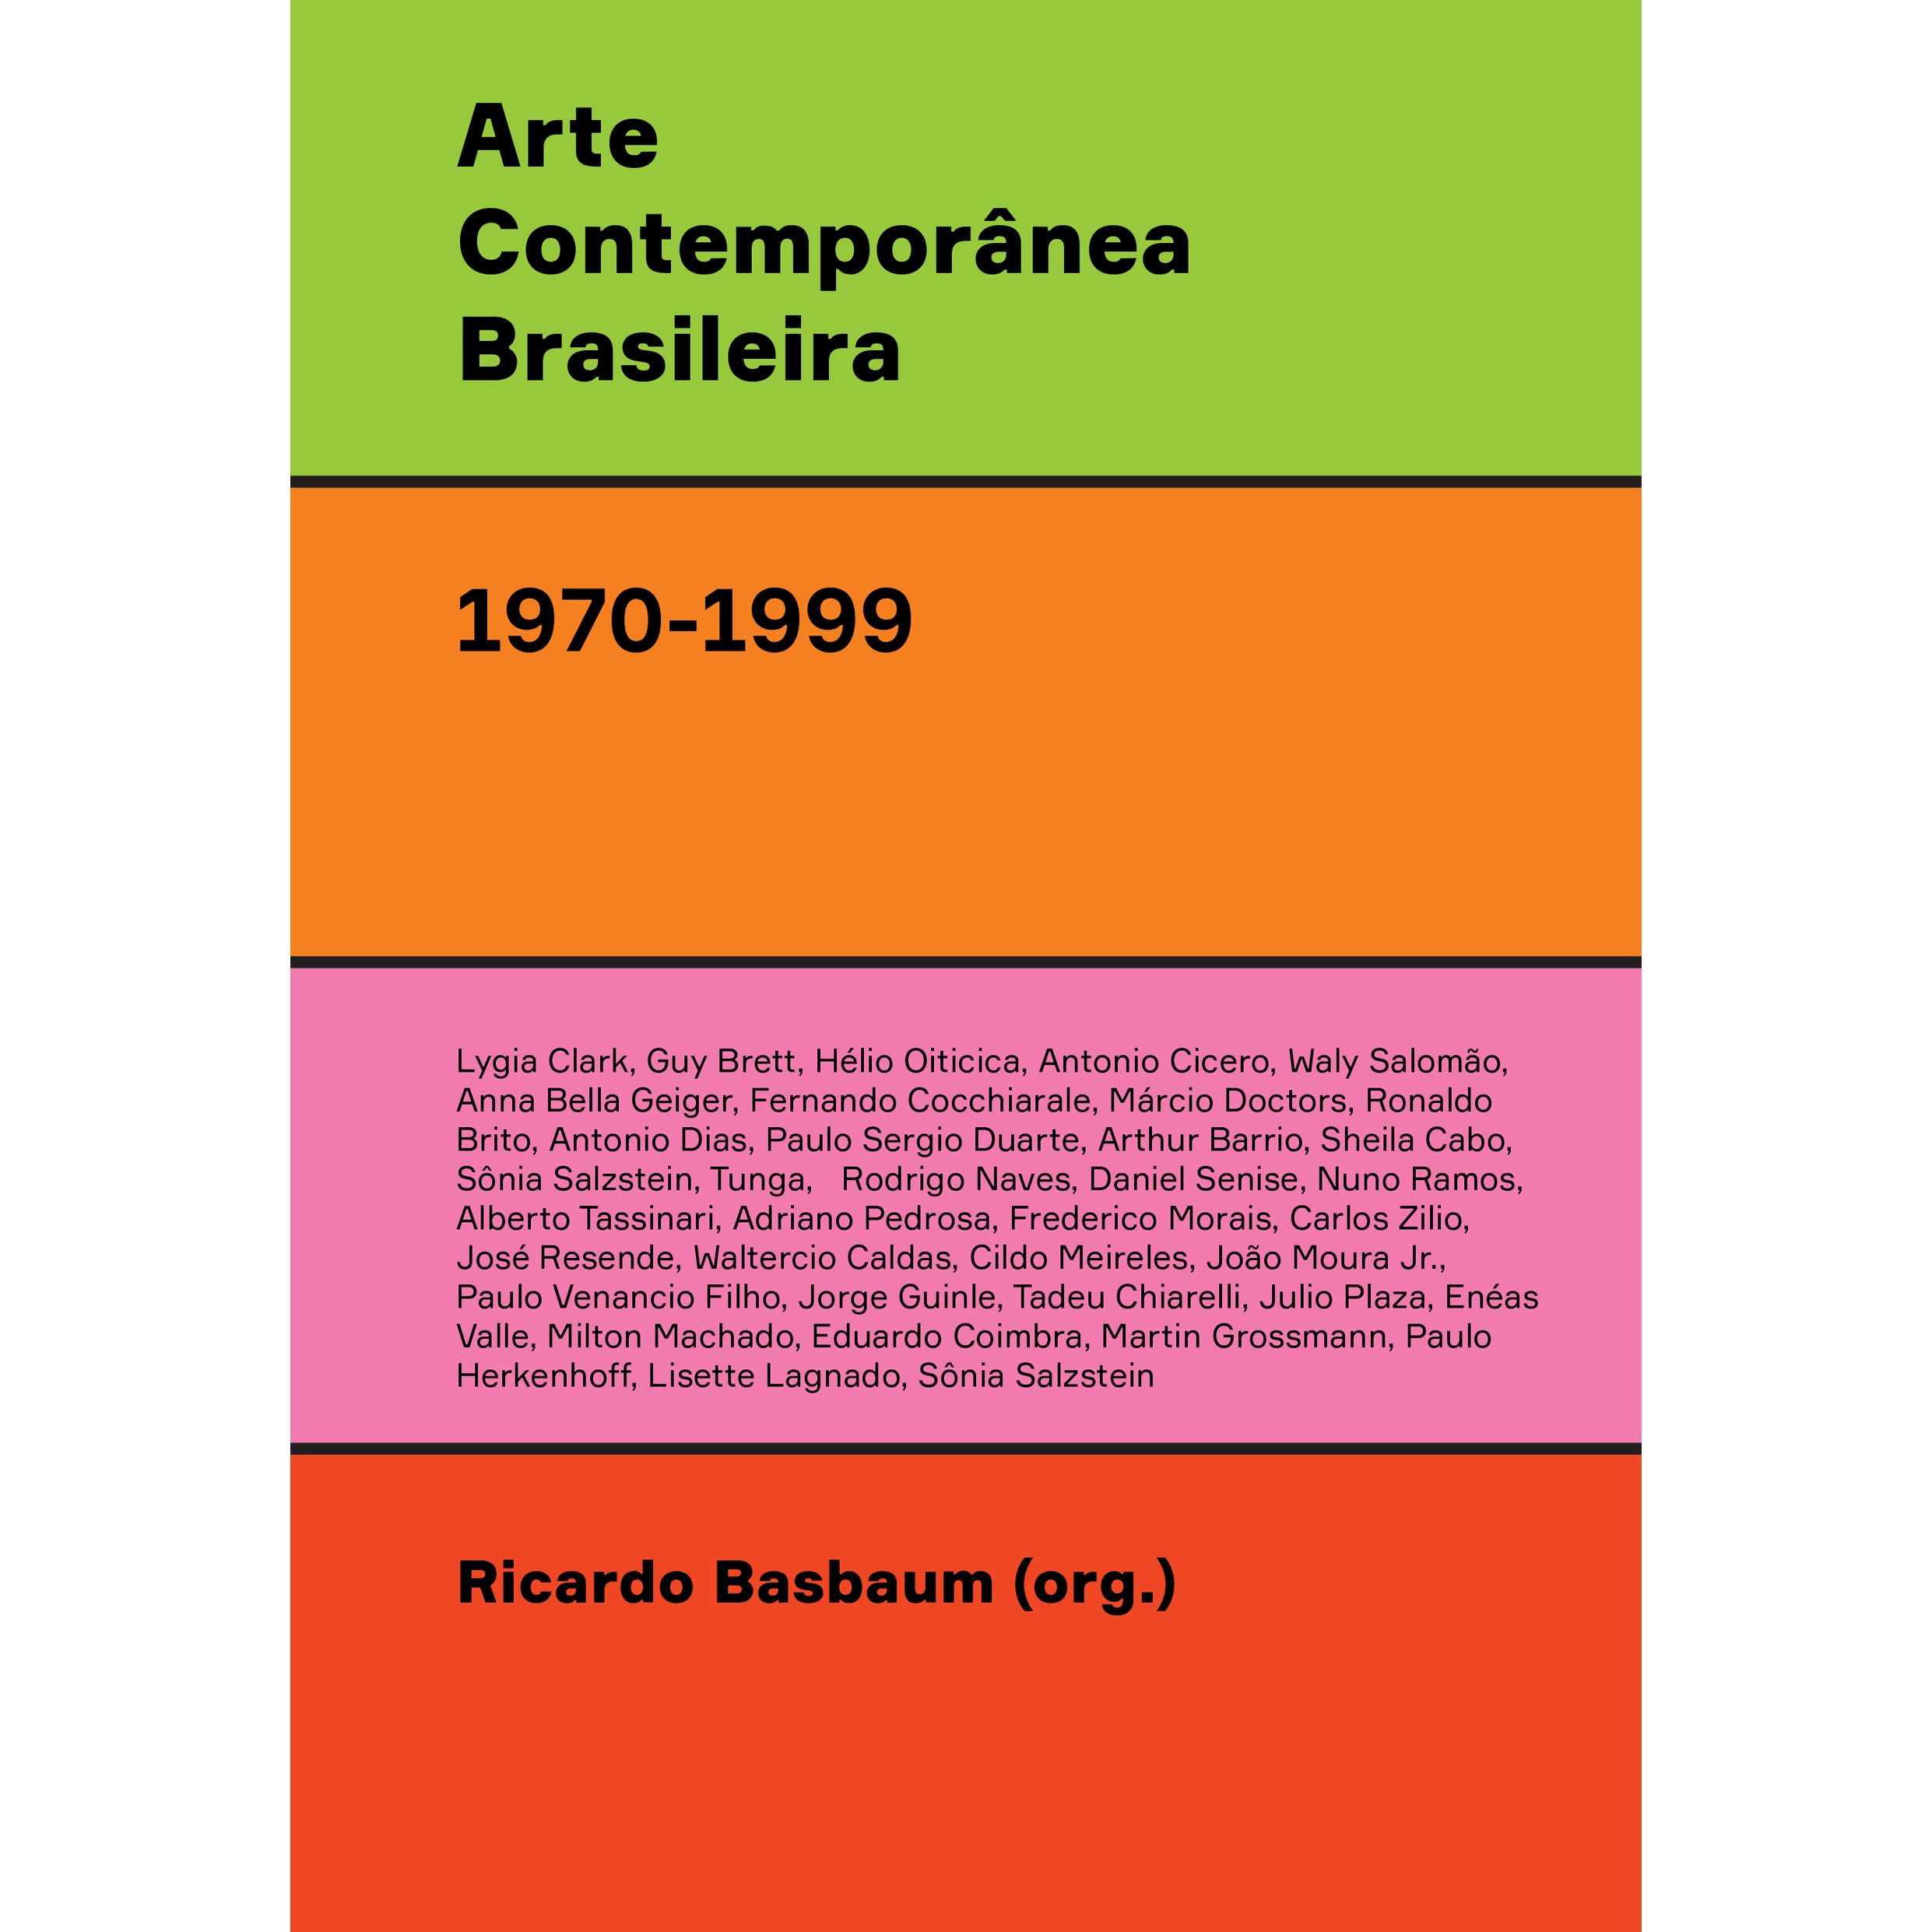
\includegraphics[width=74mm]{./CAPAS/CIRCUITO_BASBAUM.jpg}
\end{center}
\hspace*{-7cm}\hrulefill\hspace*{-7cm}
\medskip

\noindent{}A publicação de uma segunda edição de \textit{Arte contemporânea brasileira: texturas, dicções, ficções, estratégias} é, sem dúvida, \hlc{sinal indicativo de que o interesse nas questões trazidas pelo livro permanece em aberto: existiria, ainda, relevância no debate em torno da crítica de arte; seria preciso prestar atenção na presença de uma economia discursiva própria do campo da arte contemporânea} --- dinâmicas cuja operatividade desempenharia papéis-chave nas relações que se quer estabelecer com as obras e o circuito, o tecido cultural e as urgências políticas. Amplamente, a presença variada e múltipla da textualidade nos debates compartilhados do campo da arte seria portadora de engajamento, intervenção, provocação e desvio, ao mesmo tempo em que inscreve e estratifica camadas de uma geografia comum da fala e da escrita.

\vfill
\noindent\begin{minipage}[c]{1\linewidth}
{\small\textbf{
\hspace*{-.1cm}Editora: Circuito \& Hedra\\
Título: História da arte contemporânea (Vol.\,1)\\
Autor: Ricardo Basbaum (org.)\\ 
ISBN: 978-65-89705-32-1\\
Páginas: 494 (provisório)\\
Formato: 16x23\,cm\\
Preço: R\$ 179,90 (provisório)\\
}}
\end{minipage}
\pagebreak

\begin{center}
\hspace*{.5cm}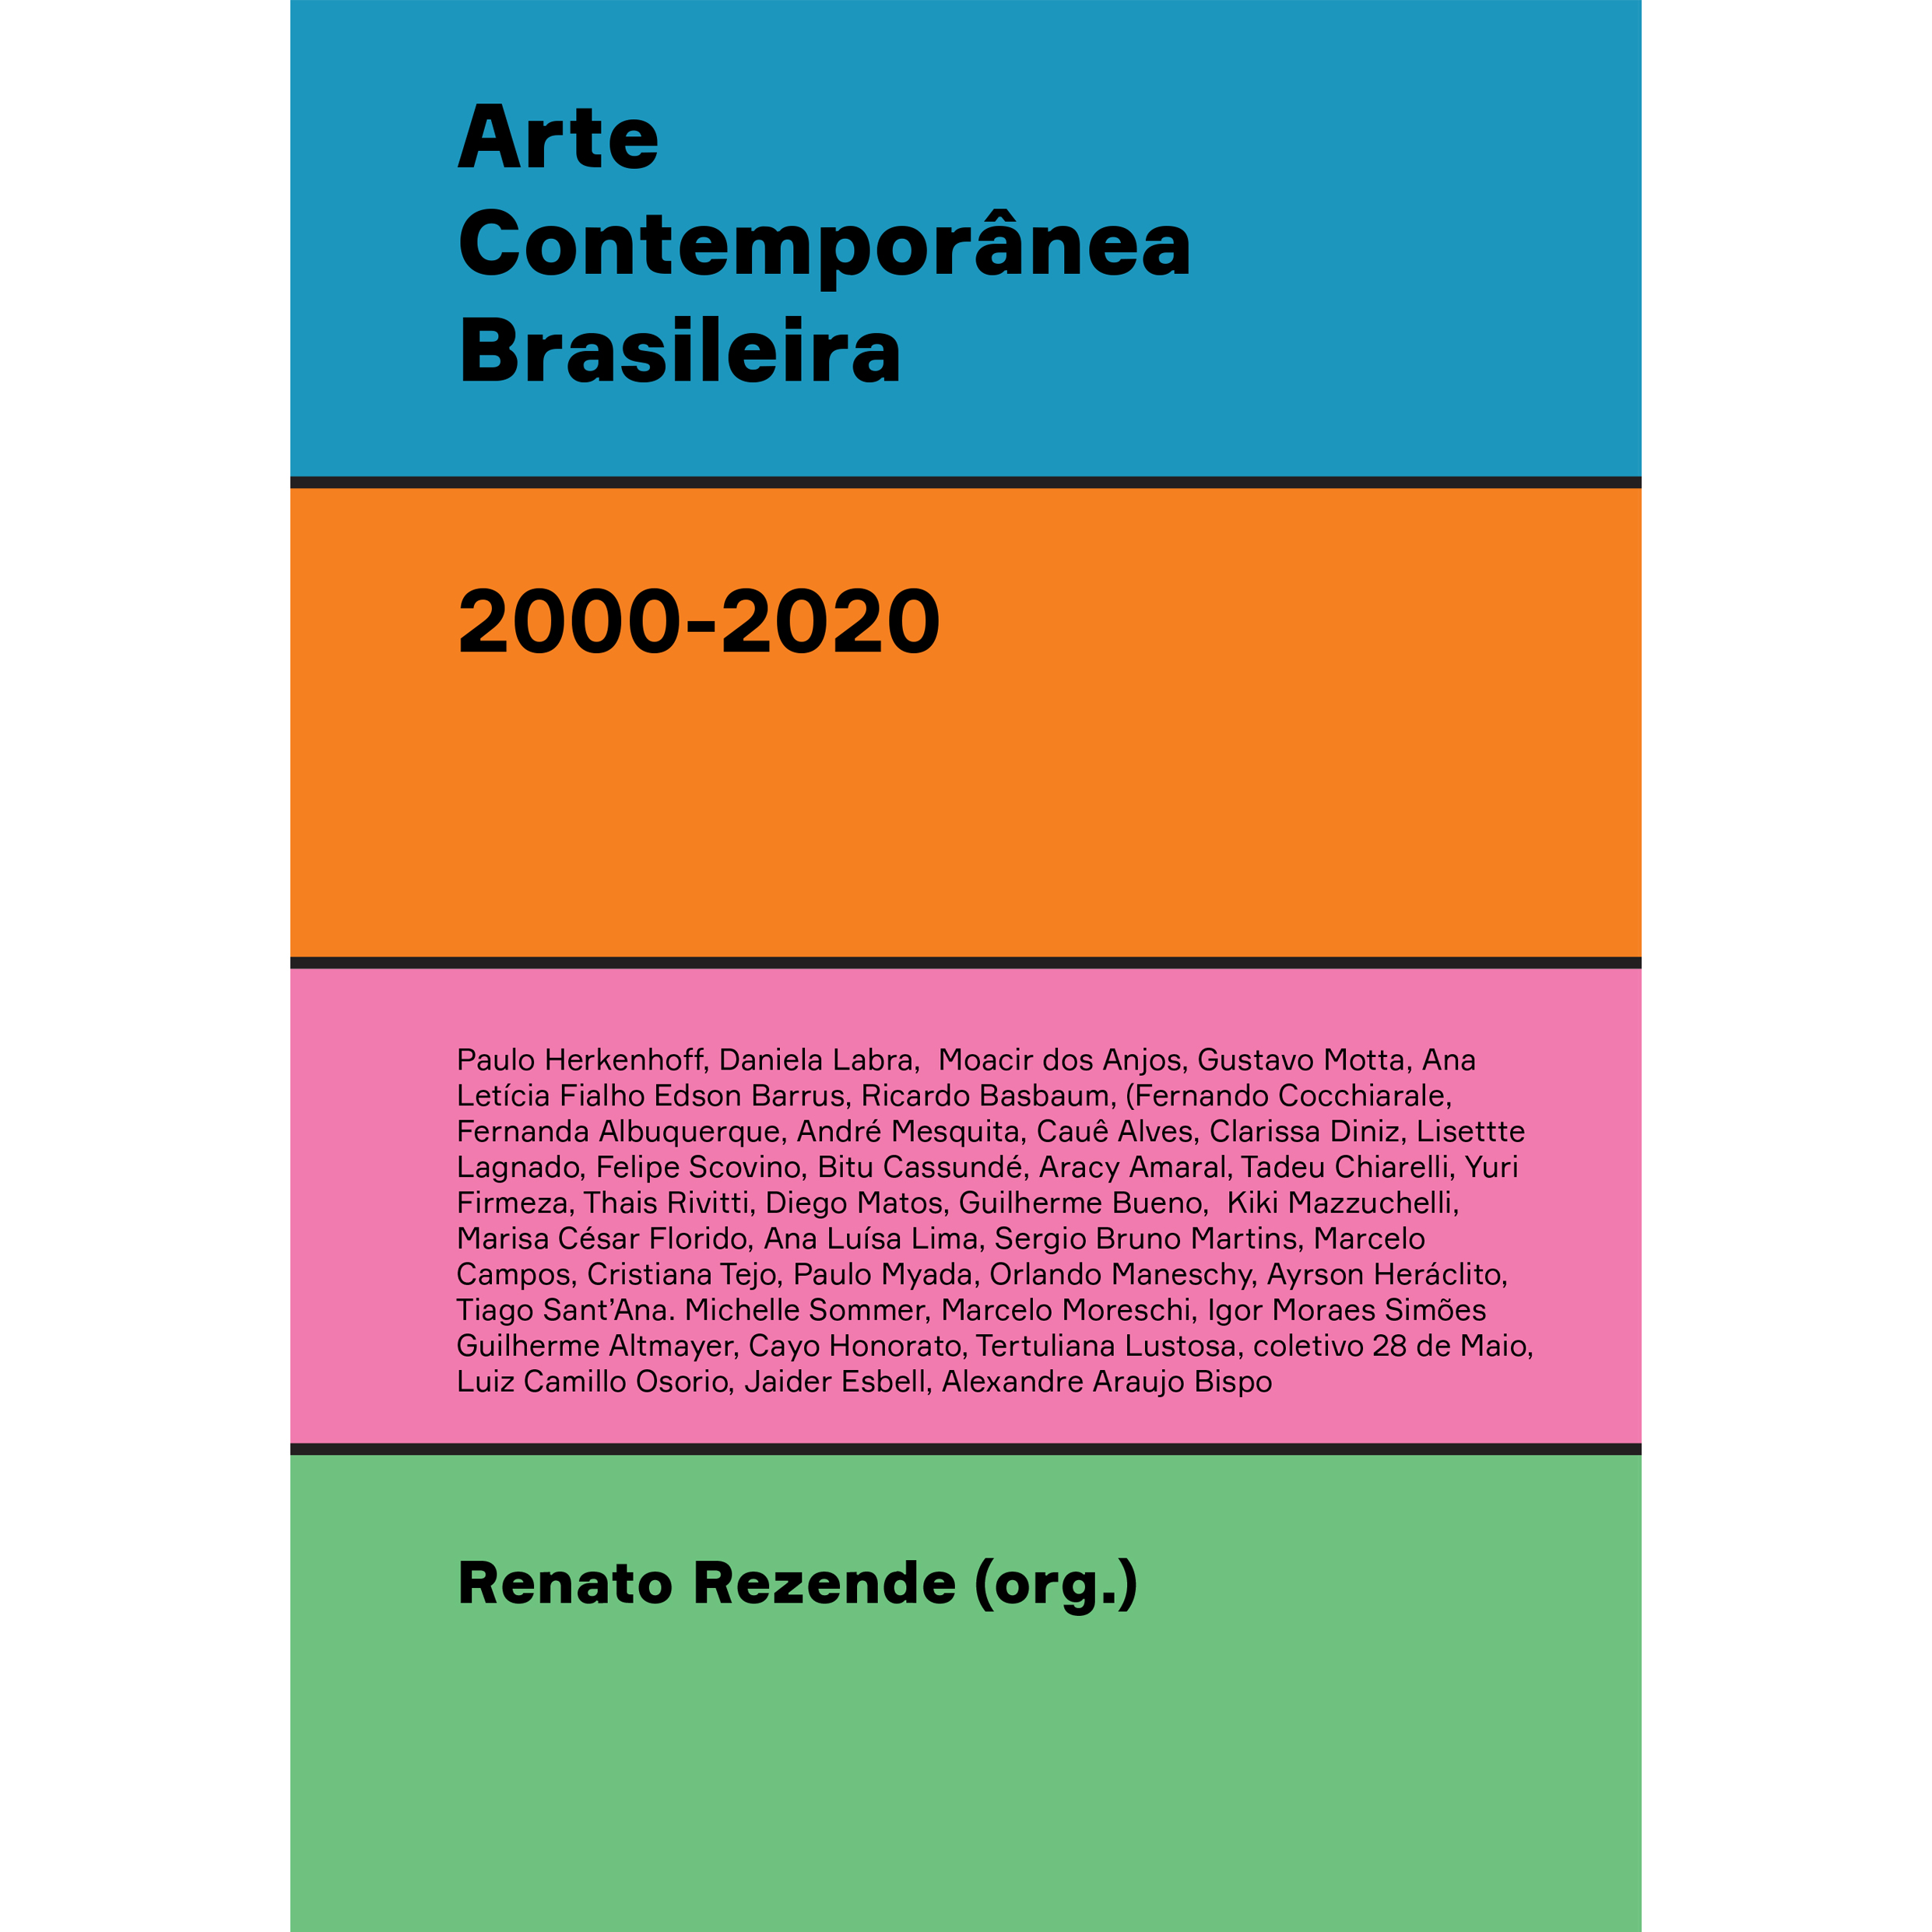
\includegraphics[width=74mm]{./CAPAS/CIRCUITO_REZENDE.jpg}
\end{center}
\hspace*{-7cm}\hrulefill\hspace*{-7cm}
\medskip

\noindent{}Tendo como recorte um período especialmente frutífero da arte visual brasileira, esta antologia se apresenta como uma espécie de percurso, no qual espera-se que o saldo final revele algo mais instigante, abundante e reflexivo que uma mera compilação de textos avulsos. \hlc{São ensaios que dialogam entre si, complementando-se, escritos por artistas, pesquisadores, críticos e curadores de arte em plena atividade. Imaginamos o livro como um mapa, abreviado e conciso, mas indicativo de um território vasto e vibrante: a produção crítico-teórica sobre a arte contemporânea brasileira nas primeiras duas décadas do século \textsc{xxi}.} De 2000 a 2020: o arco histórico que abrange parte dos anos \textsc{fhc} e os governos petistas de Lula e Dilma, incluindo as manifestações de 2013 e suas consequências imediatas até o primeiro ano do governo atual --- uma perversa ruptura que exige da arte (e da sociedade como um todo) atenção e ativa militância.

\vfill
\noindent\begin{minipage}[c]{1\linewidth}
{\small\textbf{
\hspace*{-.1cm}Editora: Circuito \& Hedra\\
Título: História da arte contemporânea (Vol.\,2)\\
Autor: Renato Rezende (org.)\\ 
ISBN: 978-65-89705-33-8\\
Páginas: 642 (provisório)\\
Formato: 16x23\,cm\\
Preço: R\$ 228,90 (provisório)\\
}}
\end{minipage}
\pagebreak

\begin{center}
\hspace*{-3.6cm}\raisebox{5cm}{\rotatebox[origin=t]{90}{\huge\textbf{Lançamento}}}
\hspace*{3.1cm}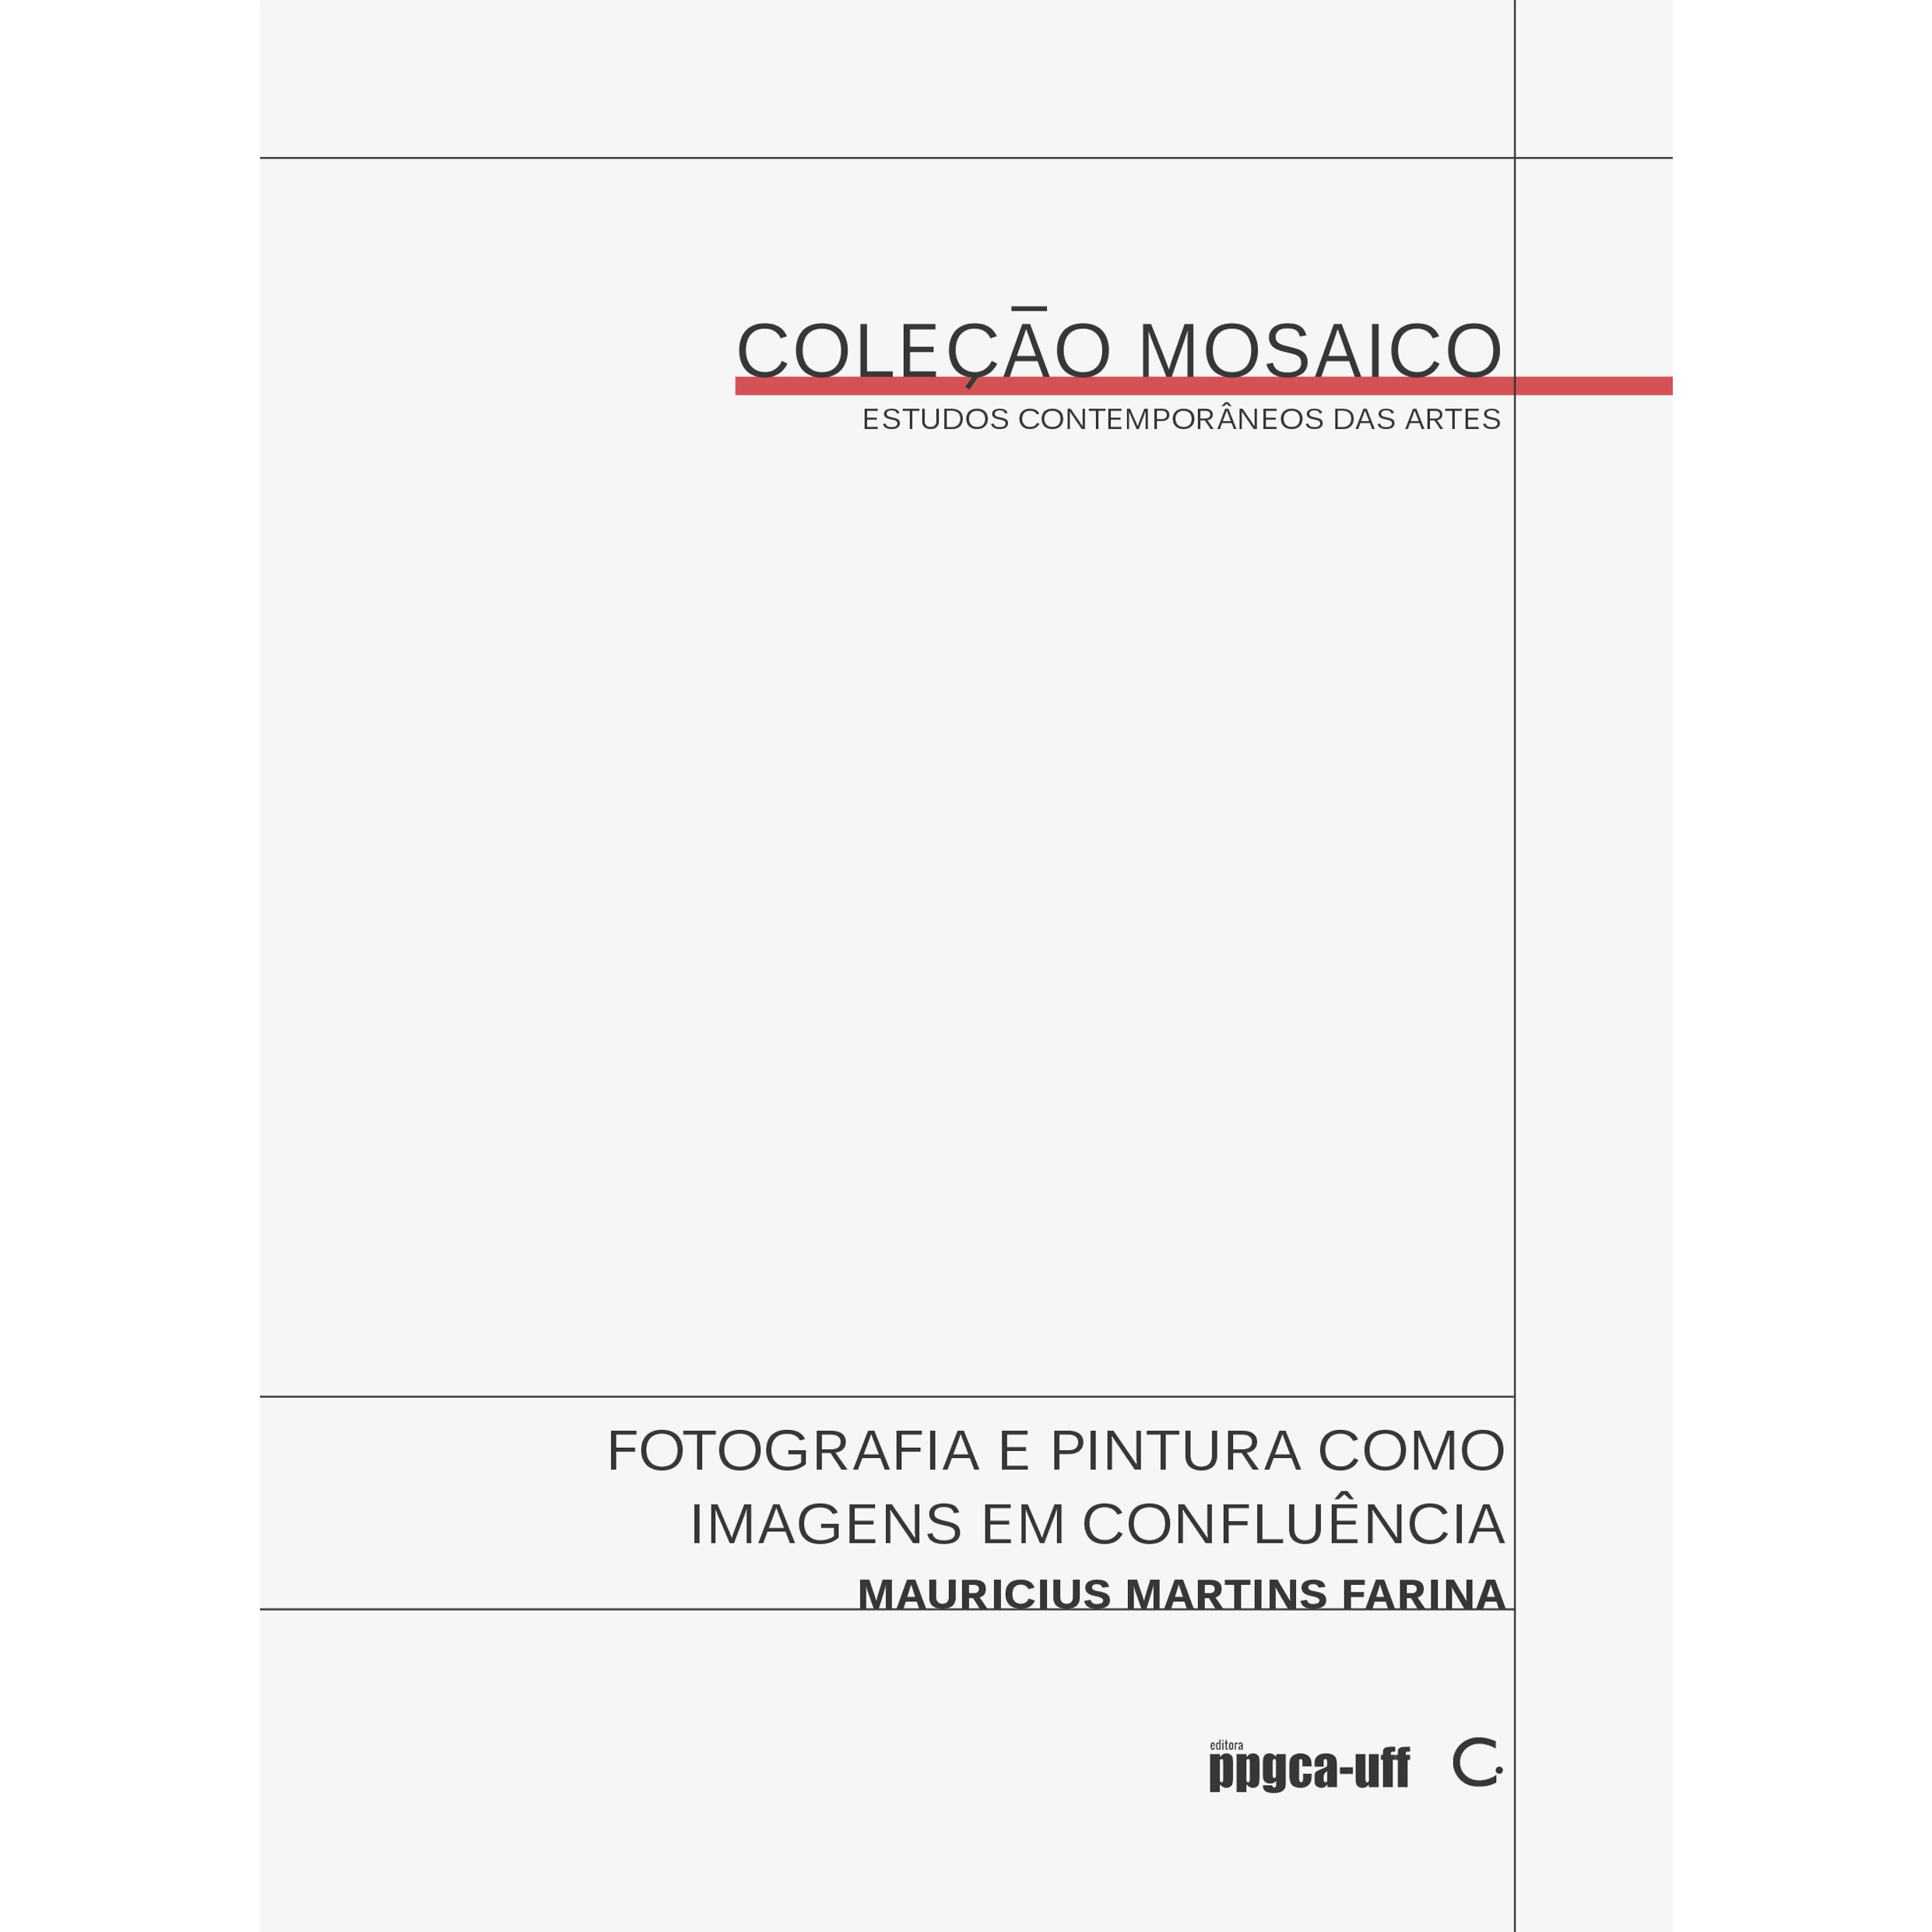
\includegraphics[width=74mm]{./CAPAS/CIRCUITO_FOTOGRAFIA.jpg}
\end{center}
\hspace*{-7cm}\hrulefill\hspace*{-7cm}
\medskip

\noindent{}A coleção Mosaico: Estudos Contemporâneos das Artes é destinada à circulação das pesquisas originais em torno da \hlc{produção das artes visuais, dança, teatro, música, artes digitais, cinema e performance.} São produções de autores nacionais ou estrangeiros, que tratam de questões pertinentes às artes na contemporaneidade de forma substantiva, a partir de uma perspectiva transdisciplinar. 

Vinculada ao Programa de Pós-Graduação em Estudos Contemporâneos das Artes da Universidade Federal Fluminense (PPGCA--UFF), é consistente com o compromisso de contribuir para a geração e circulação do PPGCA--UFF através de sua própria editora e da Circuito.

\vfill
\noindent\begin{minipage}[c]{1\linewidth}
{\small\textbf{
\hspace*{-.1cm}Editora: Circuito\\
Título: Fotografia e pintura como imagens em confluência\\
Autor: Mauricius Martins Farina\\ 
ISBN: 978-65-86974-14-0\\
Páginas: 135\\
Formato: 19x13,5\,cm\\
Preço: R\$ 49,90\\
}}
\end{minipage}
\pagebreak

\begin{center}
\hspace*{.5cm}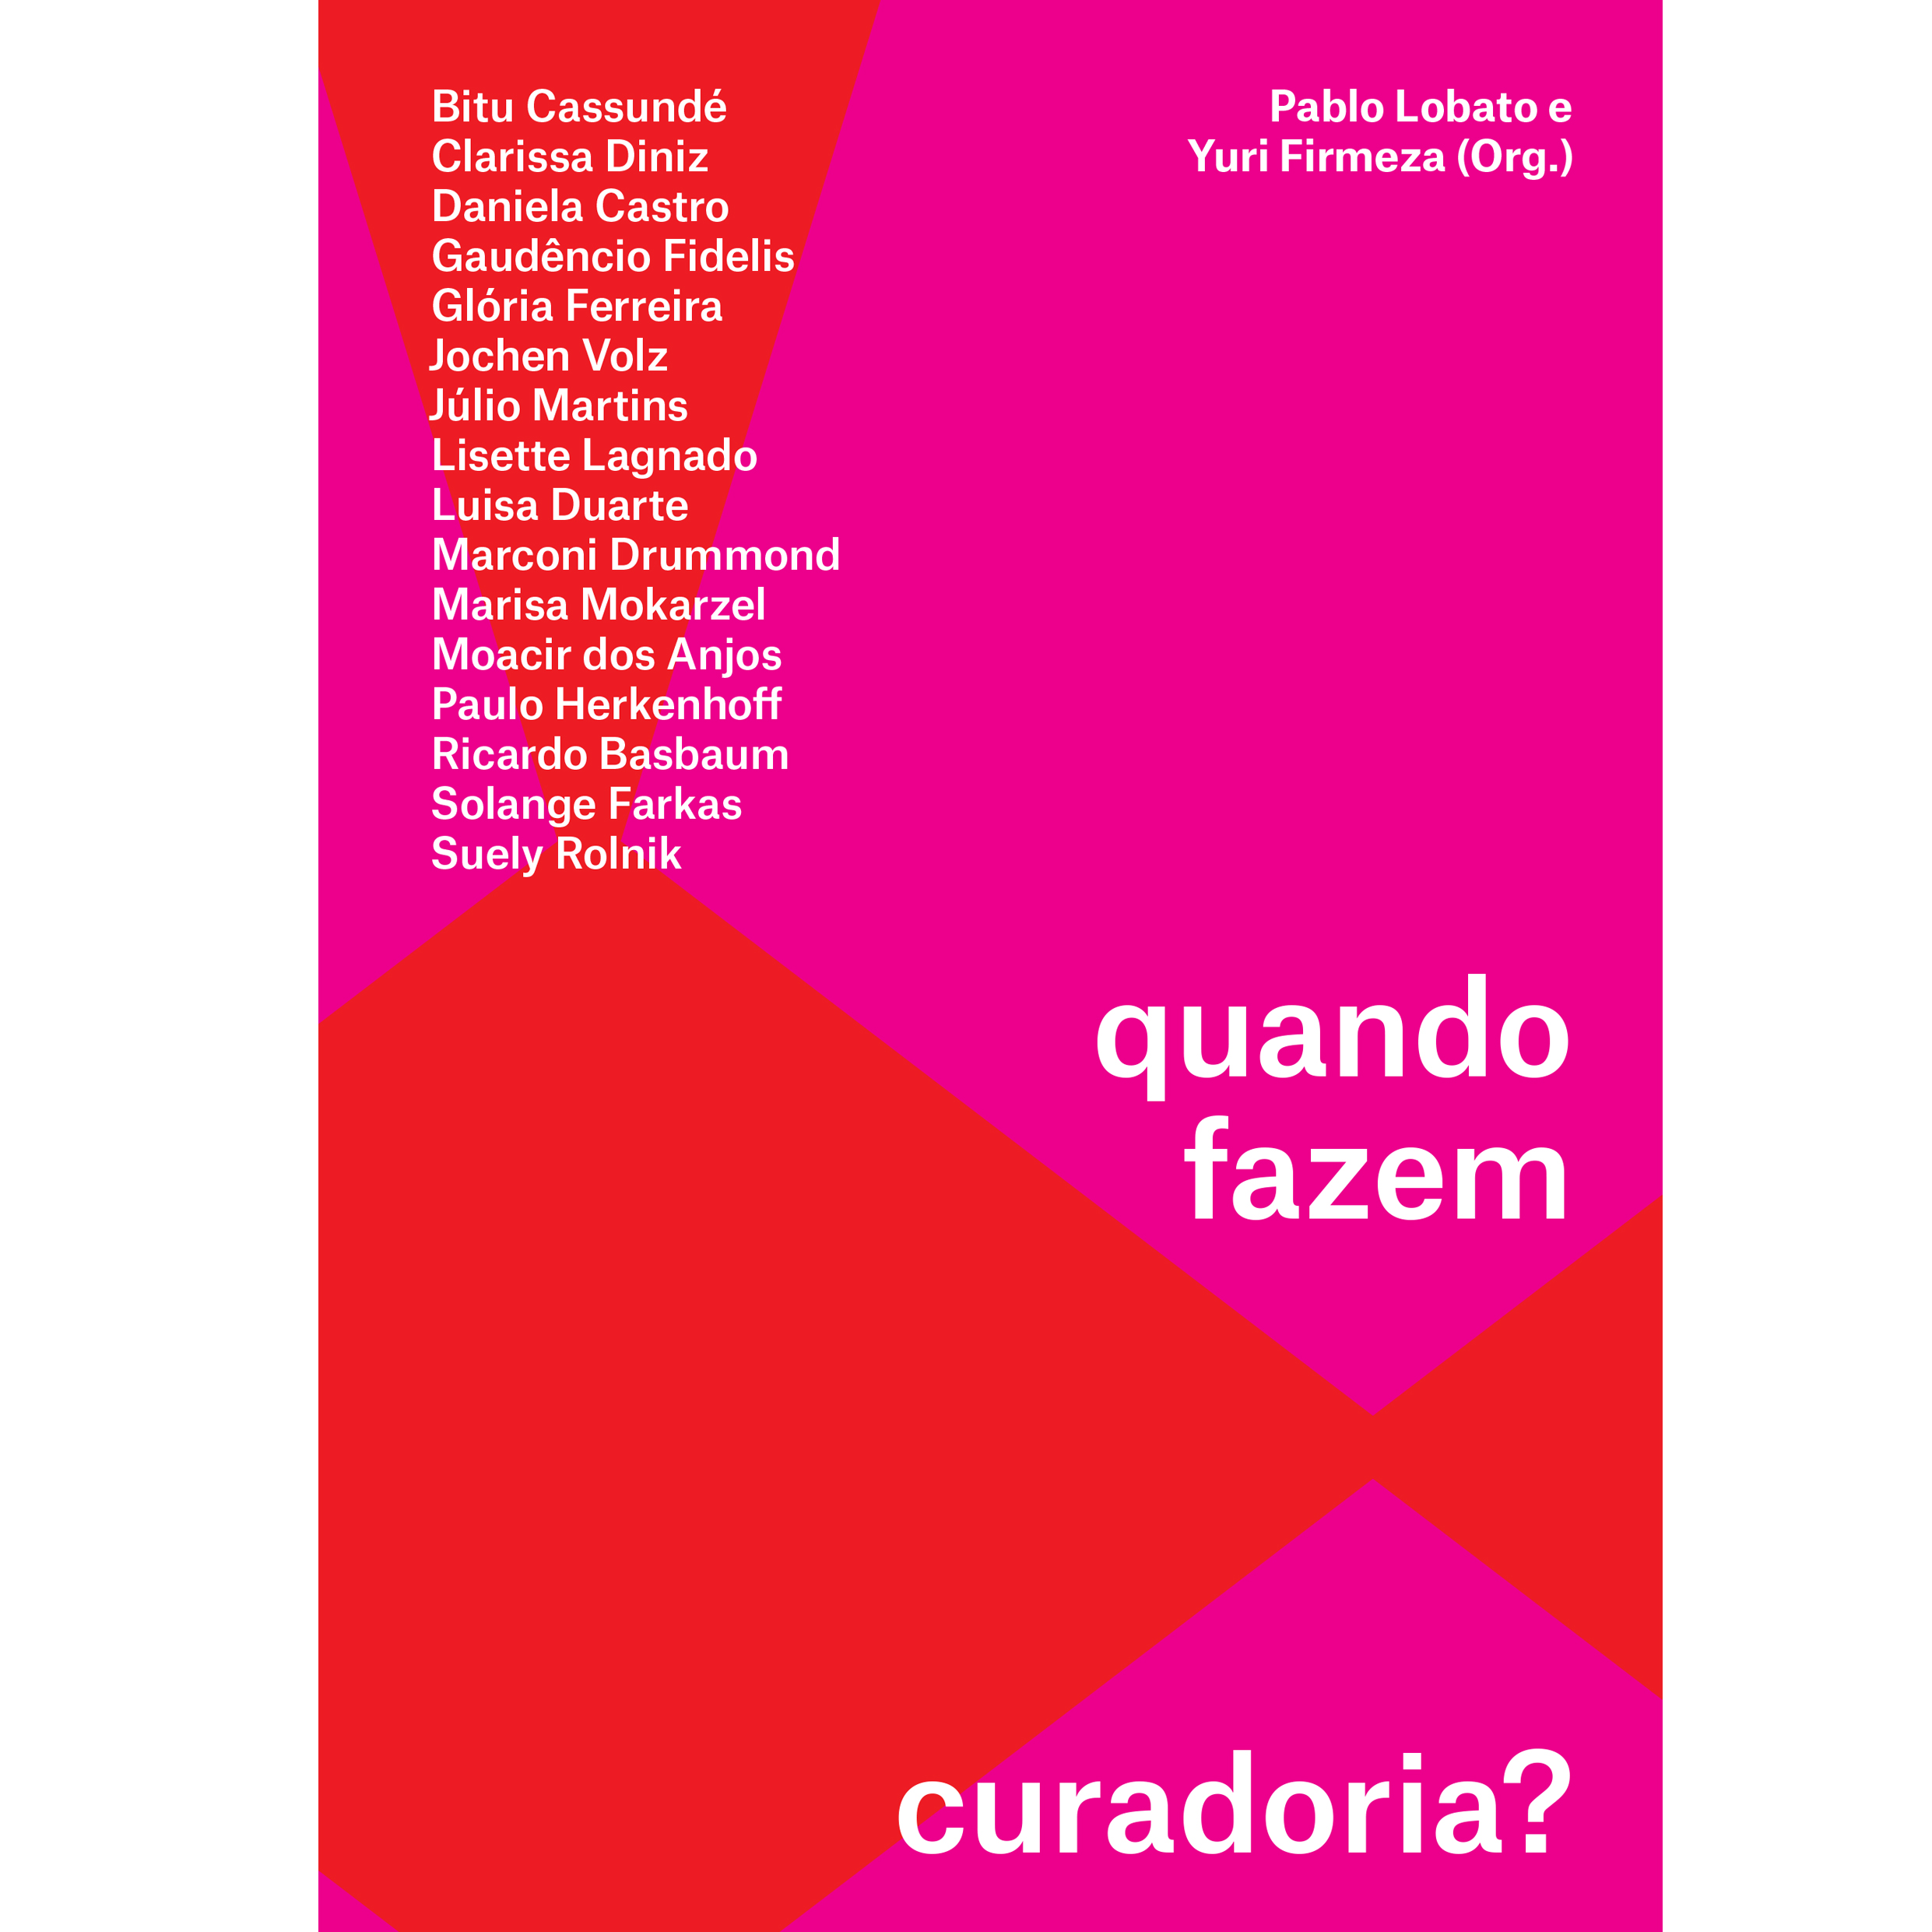
\includegraphics[width=74mm]{./CAPAS/CIRCUITO_CURADORIA.jpg}
\end{center}
\hspace*{-7cm}\hrulefill\hspace*{-7cm}
\medskip

\noindent{}A escolha dos 16 curadores que compõem o trabalho foi pautada, majoritariamente, pelas relações já existentes antes aos encontros para a produção da obra --- embora, eventualmente, um curador tenha indicado outro para integrar a conversa. \hlc{O convite, em forma de pergunta, diferente de uma entrevista, acaba por lançar cada uma das 16 sensibilidades em uma roda de confluências, multifacetada.} As respostas seriam inicialmente curtas, mas o resultado final foi uma surpresa.

\vfill
\noindent\begin{minipage}[c]{1\linewidth}
{\small\textbf{
\hspace*{-.1cm}Editora: Circuito\\
Título: O que exatamente vocês fazem?\\
Autor: Pablo Lobato \& Yuri Firmeza (orgs.)\\ 
ISBN: 978-65-86974-13-3\\
Páginas: 168\\
Formato: 14x21\,cm\\
Preço: R\$ 50,00\\
}}
\end{minipage}
\pagebreak

\vspace*{1.5cm}
\noindent{}{\nohyphens{\LARGE{Uma análise sobre as \textit{Máscaras sensoriais}\\ de Lygia Clark}}}
\bigskip

\hfill{}\scalebox{.8}{GUY BRETT}
\bigskip
\bigskip
\bigskip

\begin{multicols}{2}

\noindent{}Podemos tomar um grupo de obras de Lygia Clark\index{Clark, Lygia} do fim dos anos 1960 como eixo: as \textit{Máscaras sensoriais} (1967), e as séries de trabalhos seguintes, as \textit{Máscaras"-abismo} (1968). Eles permitem olhar ao mesmo tempo para trás, vendo a posição que Lygia alcançara naquele momento em relação a seus contemporâneos, e para diante, focalizando suas descobertas posteriores na área que ela chamou, de modo geral, \textit{nostalgia do corpo}.

As \textit{Máscaras sensoriais} são máscaras largas de pano nas quais a artista costurou objetos ou materiais que cobrem olhos e ouvidos e, no lado avesso, abaixo do nariz, uma substância aromática. A combinação de sensações, de beleza sutil, é produzida por meios simples: por exemplo, o som de uma esfera sólida rolando num pequeno recipiente contra o ouvido, talhos estreitos na altura dos olhos e uma erva aromática no nariz. Ou uma suave rede de musselina sobre os olhos, guizos em redes junto aos ouvidos e outro aroma para o olfato. Embora, para aquele que põe uma das \textit{Máscaras}, a experiência seja interna, elas ainda têm um aspecto externo para quem olha: parecem cabeças de estranhas criaturas ou capuzes vestidos por penitentes em rituais religiosos medievais. 

Com as \textit{Máscaras"-abismo}, não há aspecto externo exceto uma vaga monstruosidade. Como o nome sugere, elas são radicalmente internas. Uma venda cobre os olhos. Pendendo de um arreio na cabeça, estão sacos plásticos superinflados cercados por redes e vergados por pedras, também contidas em redes ou suspensas por elásticos. As pessoas que vestem as máscaras, sozinhas ou em grupos, tocam ou apertam os braços em volta do leve peso dos sacos de ar. ``No momento em que se respira dentro dos sacos plásticos, descobre"-se espaço {[}dentro{]} da gente e também o espaço exterior a gente''\footnote{\textsc{clark}, Lygia. ``Carta a Guy Brett\index{Brett, Guy}''. Paris, 10 de novembro de 1968}.

Vários processos foram se encadeando desde o início do trabalho de Lygia
Clark\index{Clark, Lygia} para que ela chegasse a esse ponto. Ela saiu gradualmente do
espaço privilegiado, fictício e isolado da arte para ocupar um espaço
``cotidiano'', não previamente valorizado ou articulado artisticamente.
Seus primeiros relevos foram pendurados na parede como pinturas. Sua
descida rumo ao chão torna"-se internamente articulada e convida o
espectador a atravessar uma barreira comportamental (e mesmo
terminológica) e jogar com eles. 

\vspace{\baselineskip}
{\small\fakereceipt{
\noindent{}As inovações de Lygia Clark tiveram implicações de longo alcance. Na cultura ocidental moderna, nosso modo usual de ver foi decisivamente influenciado por um processo histórico que separou o ato de ver do corpo físico do observador, numa visão sem corpo.}}
\vspace{\baselineskip}

Formas rígidas tomam"-se elásticas,
perdem sua monumentalidade autônoma e tornam"-se desenraizadas ou
permeáveis ao ambiente, amontoadas no solo, grudadas numa caixa ou num
galho (Lygia se divertiu quando Mário Pedrosa\index{Pedrosa, Mário} exclamou ao ver pela
primeira vez sua \textit{Obra mole}: ``Finalmente, uma escultura que se
pode chutar!''). Com as \textit{Máscaras sensoriais} esse processo
alcançou um novo estágio: o objeto não estava mais ``fora'' do corpo,
mas agarrado a ele, tornando"-se não um objeto apreendido pelos sentidos,
mas um filtro sensorial através do qual o mundo é experienciado.

Junto desse, outro processo provocantemente paradoxal para um artista
visual estava em desenvolvimento desde o início: a perda progressiva da
ênfase no sentido visual. Os primeiros relevos eram objetos para os
olhos. Os \textit{Bichos} introduziram o tato. As \textit{Máscaras
sensoriais} igualaram visão, audição e olfato num conjunto
plurissensorial. Na época das \textit{Máscaras"-abismo} o sentido da visão
foi completamente bloqueado e a ênfase passou de modo radical para o
corpo como um todo. Esses trabalhos ainda são chamados ``máscaras'',
cobrem o rosto e envolvem a cabeça, mas esta \textit{submerge} no corpo,
assim como, pouco antes, as \textit{Máscaras sensoriais} afundavam os
olhos nos outros sentidos. (É revelador, desse ponto de vista, que uma
\textit{Máscara sensorial} sem elementos para o ouvido e o nariz tivesse
espelhos e peças para os olhos, de modo que se pudesse mirar os próprios
olhos).

As inovações de Lygia Clark\index{Clark, Lygia} tiveram implicações de longo alcance. De
acordo com uma recente e perceptiva análise da natureza da
``visualidade'' na cultura ocidental moderna, nosso modo usual de ver
foi decisivamente influenciado por um processo histórico que ``separou o
ato de ver do corpo físico do observador, numa visão sem
corpo''\footnote{\index{Crary, Jonathan}\textsc{crary}, Jonathan. \textit{Techniques of observation: on
vision and modernity in the Nineteenth Century}. Cambridge: \textsc{mit} Press,
  1990, p. 39.}. No livro \textit{Techniques of observation: on vision and modernity in the Nineteenth Century}, Jonathan Crary analisa
minuciosamente esse fenômeno, tomando a invenção da \textit{câmera
obscura}, no século \textsc{xvi}, como um momento decisivo. Essa invenção
redefiniu radicalmente a relação entre o observador e o mundo. 

Pela
criação de um ``quarto escuro'', no qual uma imagem ótica plana do mundo
é projetada para a contemplação, o observador é impelido a ``um tipo de
\textit{askesis}, ou retirada do mundo, a fim de regular e purificar sua
relação com os conteúdos múltiplos do agora mundo `exterior'\,''\footnote{Ibid.}.
Crary relaciona esse fenômeno com um tipo mais amplo de separação
filosófica entre sujeito e objeto, conhecedor e conhecido e, em última
instância, indivíduo e cosmos. 

% Isso torna fascinante interpretar os
% experimentos de Lygia Clark\index{Clark, Lygia} dos anos 1960 como um esforço pioneiro de
% reintegrar a percepção visual e o corpo num todo, para reconectar o
% mundo interior e o exterior, o conhecedor e o conhecido.

Essas interpretações são reforçadas pelo modo como os trabalhos de Lygia
Clark\index{Clark, Lygia} representaram um desenvolvimento revolucionário das posições
alcançadas pela vanguarda do século \textsc{xx}. O impacto total dessas ideias no
Brasil coincide com o momento em que, logo depois da guerra, ela e Hélio
Oiticica\index{Oiticica, Hélio}, o outro grande inovador brasileiro, começaram a trabalhar.
Ambos viam Mondrian\index{Mondrian, Piet} e Malevitch\index{Malevitch, Kazimir} como seus mentores. Eles foram atraídos
por esses artistas porque sentiam que eram aqueles que mais
decisivamente tinham abandonado os dispositivos da representação
pictórica -- ilusionismo, profundidade, perspectiva -- herdadas do
Renascimento (para as quais a \textit{câmera obscura} foi uma ferramenta),
a fim de trabalhar com o ``espaço real do plano do quadro''. 

Contudo,
como fica claro em seus escritos e declarações, Lygia e Hélio entenderam
as realizações dos pioneiros do abstracionismo não apenas como princípio
formal e conceitual, mas também fenomenologicamente: o novo espaço
poderia, de algum modo, ser sensualmente \textit{vivido}. Pelo menos foi
dessa maneira que eles interpretaram retrospectivamente sua posição. Em
carta escrita para um amigo inglês em 1974, Hélio descreveu o
\textit{Branco sobre branco} de Malevitch em termos quase extasiados como
``um estado necessário em que as artes plásticas se despem de seus
privilégios e se \textsc{embranquecem em pele / corpo / ar}: o impulso para a
absoluta plasticidade e para o suprematismo são impulsos para a vida e
nos levam a tomar nosso \textsc{corpo} (a descobri"-lo) como a sonda da
vida''\footnote{\textsc{oiticica}, Hélio. ``Carta a Edward Pope'', 17 de agosto de
  1974. Inédita.}. Lygia Clark\index{Clark, Lygia}, referindo"-se a seus primeiros trabalhos,
contou para uma revista brasileira em 1980: ``Comecei com geometria, mas
estava procurando um espaço orgânico onde se pudesse entrar no
quadro''\footnote{\textsc{clark}, Lygia. \textit{Veja}. Rio de Janeiro, dezembro de
  1986.}.

Essas palavras iluminam a tensão dialética bem no início de sua obra, no
fim dos anos 1950, quando ela ainda usava um formato pictórico. As
séries de pinturas relevo denominadas \textit{Unidade}, por exemplo, criam
um sentido máximo de preenchimento e espaço infinito dentro do quadro
(por meio do uso de um preto particularmente denso e opaco), e ao mesmo
tempo estendem a atenção duradoura de Mondrian\index{Mondrian, Piet} à margem do quadro, à
moldura, onde a superfície pintada encontra o resto do mundo. Ligando
partes da área preta com um raso sulco branco, Lygia fez essa borda
parecer opticamente elástica como se os espaços interior e exterior
estivessem, um em relação ao outro, em contínua expansão e contração.
Aqui nós temos a sugestão de uma ligação entre uma experiência do espaço
apreendida opticamente e a respiração do corpo. Essa é uma conexão
especialmente fascinante por trazer à mente uma observação de Mondrian
depois do comentário particularmente prazeroso de certo espectador que
olhava uma de suas pinturas neoplásticas. O espectador simplesmente
virou"-se para Mondrian e disse: ``Eu respiro''. Relatando o incidente numa
carta a um amigo, Mondrian escreveu: ``Para mim é exatamente o que
deveria ser, isto é, que se respira, se sente livre, no ato de olhar
para uma tela.''\footnote{\textsc{mondrian}, Piet. In: \textsc{matthes}, Hendrik. ``Aphorisms\index{Matthes, Hendrik}
  and reflections by Piet Mondrian\index{Mondrian, Piet}'', \textit{Kunst \& Museum Journal},
  vol. 6, n. I, 1995, p. 57-62.}

É como se ele fizesse o roteiro para a viagem de Lygia Clark\index{Clark, Lygia} além do
óptico. Em 1967 Lygia fez uma de suas mais belas proposições
simples/\,complexas, \textit{Respire comigo}. Pega"-se um tubo de borracha de
curta extensão (tirado do equipamento de oxigênio dos mergulhadores),
junta"-se as duas pontas de modo que um canal seja produzido, coloca"-se o
polegar sobre o canal e dilata"-se o tubo para fazer um som de respiração
no próprio ouvido. É como se alguém tirasse o pulmão do próprio peito ou
evocasse uma outra pessoa intimamente próxima. Lygia escreveu sobre suas
\textit{Máscaras}-\textit{abismo} na carta de 1968 citada anteriormente:

\begin{quote}
Elas têm o mesmo sentido que \textit{Respire comigo}, porque quero que as
pessoas o façam por si mesmas, e no momento em que se respira dentro dos
sacos plásticos descobre"-se um espaço {[}dentro{]} de si e também o
espaço exterior da gente. Organicidade, o inteiro vazio, todos os
conceitos que propus antes no objeto estão agora introvertidos no
interior da pessoa. Homem, objeto de si mesmo, como diz Mario
\index{Pedrosa, Mário}Pedrosa.\footnote{\textsc{clark}, Lygia. ``Carta a Guy Brett''. Paris, 10 de
  novembro de 1968.}\index{Brett, Guy}
\end{quote}

Em outras palavras, Lygia chegou a um ponto em que o vazio, o espaço de
projeção, alcançado no desenvolvimento da arte abstrata no século \textsc{xx},
foi abraçado, engolido, incorporado pelo objeto da comunicação
artística, o espectador.

\bigskip
\noindent{}\textcolor{gray}{\footnotesize\slsc{\textls[-15]{Adaptação de capítulo \textit{Lygia Clark: seis céulas}, presente no volume “Arte contemporânea brasileira (1970--1999)”.}}}
\end{multicols}

\pagebreak
\pagestyle{circuitocat}
\begin{multicols}{2}
\begin{enumerate}
\raggedright\nohyphens{
\item Introdução à Soma \textbf{João da Mata}
\item Filosofia Black Bloc \textbf{Murilo Duarte Costa Correa}
\item 2013 \textbf{Camila Jourdan}
\item Antifa \textbf{Vários autores}
\item 1967, meio século depois \textbf{Vários autores}
\item Experimentum linguae \textbf{Giorgio Agamben}
\item Adoecer \textbf{Hélia Correia}
\item Todos os lugares \textbf{Alex Cerveny}
\item Formas híbridas \textbf{Rafael Gutiérrez}
\item Até ano que vem em Jerusalém \textbf{Maria da Conceição Caleiro}
\item Coisas que fiz e ninguém notou mas que mudaram tudo \textbf{Moisés Alves}
\item Escrever sobre escrever poesia \textbf{Eduardo Milán}
\item Noturno Europeu \textbf{Rui Nunes}
\item O tropo tropicalista \textbf{João Camillo Penna}
\item Quem apaga a luz sou eu \textbf{Magda Romano}
\item Mudança \textbf{Verónica Gerber Bicecci}
\item Fim do Infante \textbf{Marina Marcondes Machado}
\item A loucura branca \textbf{Jaime Rocha}
\item As artes do cover \textbf{Henrique Saidel}
\item Leituras furadas \textbf{Luis Felipe Fabre}
\item Éter \textbf{António Cabrita}
\item A liberação da mosca \textbf{Luigi Amara}
\item Daniel Acosta \textbf{Vários autores}
\item Café irlandês \textbf{Barbosa Lagos}
\item Escrito e dirigido por Moisés Alves \textbf{Moisés Alves}
\item Romance de asilo \textbf{André Monteiro}
\item A cena lenta \textbf{Cláudio Oliveira}
\item Frestas \textbf{André Gardel}
\item O fantasma de um nome \textbf{poesia, imaginário, vida) \textbf{Jorge Monteleone}
\item Lasca de breu \textbf{Guilherme Delgado}
}
\end{enumerate}
\end{multicols}

\pagebreak
